%%%%%%%%%%%%%%%%%%%%%%%%%%%%%%%%%%%%%%%%%%%%%%%%%%%%%%%%%%%%%%%%%%%%%%%%%%%

\documentclass{standalone}

\usepackage{amsmath}
\usepackage{mathptmx}
\usepackage{tikz}
\usetikzlibrary{external}
\tikzexternalize{arithmetic-geometric-inequality}

%% IEEE uses Times Roman font, so we'll default to Times.
%% These three commands make up the entire times.sty package.
\renewcommand{\rmdefault}{ptm}
\renewcommand{\ttdefault}{pcr}
\normalfont\selectfont

%%%%%%%%%%%%%%%%%%%%%%%%%%%%%%%%%%%%%%%%%%%%%%%%%%%%%%%%%%%%%%%%%%%%%%%%%%%
%% The arithmetic-mean geometric-mean inequality.
%%%%%%%%%%%%%%%%%%%%%%%%%%%%%%%%%%%%%%%%%%%%%%%%%%%%%%%%%%%%%%%%%%%%%%%%%%%

\begin{document}

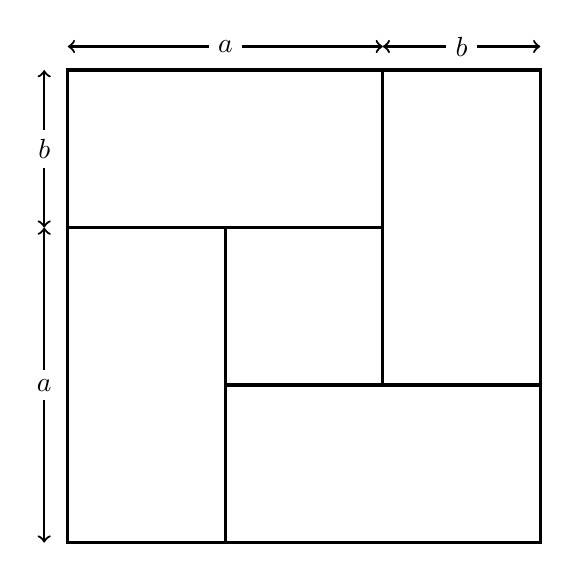
\begin{tikzpicture}[%%
  arrowStyle/.style={<->,thick},%%
  labelStyle/.style={fill=white},%%
  lineStyle/.style={-,very thick}%%
]
%%
%%
\pgfmathsetmacro{\dx}{0.3}
\pgfmathsetmacro{\dy}{\dx}
\pgfmathsetmacro{\sside}{6}
\pgfmathsetmacro{\length}{4}
\pgfmathsetmacro{\width}{2}
\pgfmathsetmacro{\xlow}{0}
\pgfmathsetmacro{\ylow}{\xlow}
%%
\coordinate (lowerLeft) at (\xlow,\ylow);
\coordinate (upperRight) at (\sside,\sside);
%%
\normalsize
%% Draw the larger square.
\draw[lineStyle] (lowerLeft) rectangle (upperRight);
%% Draw the rectangles inside the larger square.
\draw[lineStyle] (\xlow,\length) -- (\length,\length);
\draw[lineStyle] (\width,\width) -- (\sside,\width);
\draw[lineStyle] (\width,\ylow) -- (\width,\length);
\draw[lineStyle] (\length,\width) -- (\length,\sside);
%% Label the left side of the square.
\draw[arrowStyle] (-\dx,\length) -- (-\dx,\sside);
\node[labelStyle] at (-\dx,\sside-\width/2) {$b$};
\draw[arrowStyle] (-\dx,\ylow) -- (-\dx,\length);
\node[labelStyle] at (-\dx,\length/2) {$a$};
%% Label the top side of the square.
\draw[arrowStyle] (\xlow,\sside+\dy) -- (\length,\sside+\dy);
\node[labelStyle] at (\length/2,\sside+\dy) {$a$};
\draw[arrowStyle] (\length,\sside+\dy) -- (\sside,\sside+\dy);
\node[labelStyle] at (\length+\width/2,\sside+\dy) {$b$};
\end{tikzpicture}

\end{document}
